\documentclass[tikz,border=4pt]{standalone}
\usepackage{amsmath}
\begin{document}
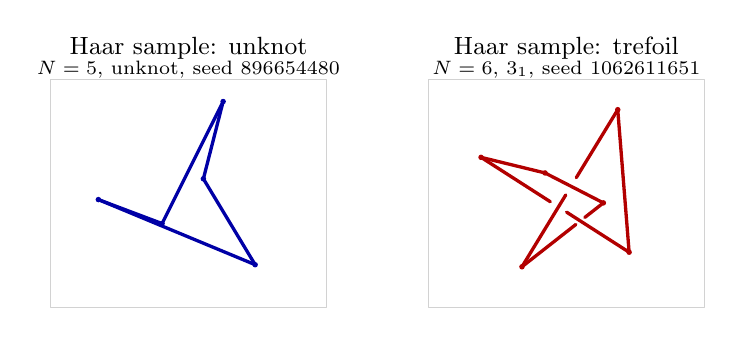
\begin{tikzpicture}[line cap=round,line join=round]
\begin{scope}[xshift=0.000cm]
\node[font=\small] at (0,1.85) {Haar sample: unknot};
\node[font=\scriptsize] at (0,1.58) {$N=5$, unknot, seed 896654480};
\draw[gray!35] (-1.75,-1.45) rectangle (1.75,1.45);
\draw[very thick,blue!65!black] (0.4408,1.1697) -- (-0.3345,-0.3804);
\draw[very thick,blue!65!black] (-0.3345,-0.3804) -- (-1.1438,-0.0754);
\draw[very thick,blue!65!black] (-1.1438,-0.0754) -- (0.8475,-0.9026);
\draw[very thick,blue!65!black] (0.8475,-0.9026) -- (0.1901,0.1887);
\draw[very thick,blue!65!black] (0.1901,0.1887) -- (0.4408,1.1697);
\fill[blue!65!black] (0.4408,1.1697) circle (0.035);
\fill[blue!65!black] (-0.3345,-0.3804) circle (0.035);
\fill[blue!65!black] (-1.1438,-0.0754) circle (0.035);
\fill[blue!65!black] (0.8475,-0.9026) circle (0.035);
\fill[blue!65!black] (0.1901,0.1887) circle (0.035);
\end{scope}
\begin{scope}[xshift=4.800cm]
\node[font=\small] at (0,1.85) {Haar sample: trefoil};
\node[font=\scriptsize] at (0,1.58) {$N=6$, $3_1$, seed 1062611651};
\draw[gray!35] (-1.75,-1.45) rectangle (1.75,1.45);
\draw[very thick,red!70!black] (-0.2712,0.2628) -- (-1.0840,0.4611);
\draw[very thick,red!70!black] (-1.0840,0.4611) -- (-0.2042,-0.1026);
\draw[very thick,red!70!black] (0.0027,-0.2352) -- (0.7969,-0.7441);
\draw[very thick,red!70!black] (0.7969,-0.7441) -- (0.6524,1.0662);
\draw[very thick,red!70!black] (0.6524,1.0662) -- (0.1260,0.2030);
\draw[very thick,red!70!black] (-0.0078,-0.0164) -- (-0.5639,-0.9286);
\draw[very thick,red!70!black] (-0.5639,-0.9286) -- (0.1204,-0.3917);
\draw[very thick,red!70!black] (0.2341,-0.3024) -- (0.4699,-0.1174);
\draw[very thick,red!70!black] (0.4699,-0.1174) -- (-0.2712,0.2628);
\fill[red!70!black] (-0.2712,0.2628) circle (0.035);
\fill[red!70!black] (-1.0840,0.4611) circle (0.035);
\fill[red!70!black] (0.7969,-0.7441) circle (0.035);
\fill[red!70!black] (0.6524,1.0662) circle (0.035);
\fill[red!70!black] (-0.5639,-0.9286) circle (0.035);
\fill[red!70!black] (0.4699,-0.1174) circle (0.035);
\end{scope}
\end{tikzpicture}
\end{document}
